\documentclass[journal]{IEEEtran}

\usepackage{cite}
\usepackage{amsmath,amssymb}
\usepackage{graphicx}
\usepackage{array}
\usepackage{booktabs}
\usepackage{url}
\usepackage{seqsplit}
\usepackage{balance}
\usepackage[hidelinks]{hyperref}

\graphicspath{{figures/}}
\DeclareGraphicsExtensions{.pdf,.png,.jpg}

\newcommand{\TL}{\texttt{transport\_logistics4}}
\newcommand{\URB}{\texttt{urban\_structural4}}
\newcommand{\NoEnt}{\texttt{No-Ent}}
\newcommand{\ZZRA}{\texttt{ZZ+RA}}

\begin{document}

\title{Regime-Bounded Metrics for Qiskit Hybrid Quantum Heads in Low-Shot Remote Sensing ROI Classification}

\author{Wenqi Wang$^{*\dagger}$, Lin Bi$^{*\dagger}$, Hanghang Wang$^{\S}$, and Gopal Verma$^{\ddagger}$%
\thanks{$^*$School of Computer Science and Technology, Changchun University of Science and Technology, Changchun, 130022, China.}%
\thanks{$^\dagger$Key Laboratory of Network and Information Security in Jilin Province, Changchun University of Science and Technology, Changchun, 130022, China.}%
\thanks{$^\ddagger$GPL Photonics Laboratory, Changchun Institute of Optics, Fine Mechanics and Physics, Chinese Academy of Sciences, Changchun, 130033, China.}%
\thanks{$^\S$Chang Guang Satellite Technology Co., Ltd., Changchun, China.}%
\thanks{Corresponding author: Lin Bi. E-mail addresses: jerry.neal.wang@gmail.com (Wenqi Wang), bilin@cust.edu.cn (Lin Bi), wanghanghang@jl1.cn (Hanghang Wang), and gvpal12138@gmail.com (Gopal Verma).}%
}

\markboth{IEEE Geoscience and Remote Sensing Letters,~Vol.~XX, No.~X, 2026}%
{Wang \MakeLowercase{\textit{et al.}}: Regime-Bounded Metrics for Qiskit Hybrid Quantum Heads}

\maketitle

\begin{abstract}
Hybrid quantum neural networks have been introduced into Earth-observation image analysis, but their empirical value remains difficult to interpret when the quantum branch is not compared with a matched classical control or when positive results are not bounded by stress tests. This letter reformulates the evaluation of Qiskit hybrid quantum heads as a regime-bounded measurement problem for low-shot remote sensing region-of-interest (ROI) classification. Three metrics are proposed: the quantum-classical advantage domain (QCAD), which identifies operating windows with positive paired quantum-head gains; the low-shot efficiency coefficient (LSEC), which normalizes the gain by labeled samples and runtime cost; and the quantum inductive bias (QIB), which measures whether the gain is class structured. Experiments are performed on DIOR-derived ROI crops with a four-class \TL{} subset, a 16-shot protocol, seven paired random seeds, a lightweight CNN backbone, a matched classical hybrid control, and two Qiskit quantum heads. With 16 training samples per class, the matched control obtains a macro-F1 of $0.3055\pm0.1729$, whereas the no-entanglement and ZZFeatureMap+RealAmplitudes heads reach $0.5031\pm0.1421$ and $0.4545\pm0.1735$, respectively. The advantage contracts at 32/64 shots, disappears under a ResNet18 boundary test, and does not transfer stably to \URB{}. The conclusion is therefore a context-bounded empirical gain rather than a general claim of quantum advantage.
\end{abstract}

\begin{IEEEkeywords}
DIOR, few-shot learning, hybrid quantum neural networks, low-shot remote sensing, matched control, Qiskit, quantum machine learning, region-of-interest classification.
\end{IEEEkeywords}

\section{Introduction}
Deep neural networks have become the dominant model family for remote sensing scene classification \cite{cheng2017rsi}, optical object detection \cite{li2020dior}, and large-scale aerial benchmarks such as AID, EuroSAT, and DOTA \cite{xia2017aid}, \cite{helber2019eurosat}, \cite{xia2018dota}. Broad surveys also document the shift toward deep feature learning in remote sensing \cite{zhu2017deep}. Their performance, however, typically depends on abundant annotations and strong feature extractors. In optical remote sensing, object-level ROI labels are costly: beyond manual boxing, class imbalance, and quality control, each additional batch of labeled crops also increases the experimental burden of simulating and repeatedly optimizing hybrid quantum branches.

The low-shot setting in this letter is therefore an efficiency-cost regime. A model must extract discriminative information from only a few labeled samples per class while absorbing the runtime overhead introduced by a quantum or quantum-inspired branch. Few-shot remote-sensing studies have emphasized that limited labels, class imbalance, and domain shifts should be evaluated with explicit controls \cite{qiu2024fewshot}, \cite{zhang2023gfrod}. If the same performance can be obtained by adding labels, using a stronger backbone, or training a larger classical head, the practical necessity of a compact quantum head is weakened. A meaningful hybrid-QNN claim should state not only whether a quantum head improves macro-F1, but also within which label and runtime windows that improvement remains useful.

Hybrid quantum learning builds on parameterized quantum circuits and variational optimization \cite{biamonte2017qml}, \cite{cerezo2021vqa}. Its interpretation must also account for trainability limits such as barren plateaus and noise-induced gradient suppression \cite{mcclean2018barren}, \cite{wang2021noise}, as well as feature-map views of quantum learning models \cite{havlicek2019supervised}, \cite{schuld2019feature}. Existing remote sensing QML studies show that circuit-based hybrid models can be embedded into Earth-observation pipelines \cite{sebastianelli2022circuit}, \cite{zhang2023hybrid}, \cite{fan2025hybrid}. The closest benchmark evaluates hybrid quantum CNNs for EuroSAT-style land-use/land-cover scene classification and compares circuit designs \cite{sebastianelli2022circuit}. In contrast, this letter focuses on object-level ROI crops derived from DIOR and asks a narrower question: when the backbone, projection, fusion layer, and training protocol are matched, can replacing a classical branch with a Qiskit quantum head yield a measurable low-shot gain?

The contributions are threefold. First, QCAD, LSEC, and QIB are introduced as compact boundary metrics for interpreting hybrid-QNN results in remote sensing ROI classification. Second, two Qiskit quantum heads are compared with a matched classical hybrid control over seven paired seeds, with paired Wilcoxon tests, paired bootstrap confidence intervals, per-class diagnostics, and runtime accounting. Third, the observed gain is shown to be confined to a narrow 16-shot \TL{} small-CNN simulation regime and compressed by additional labels, a stronger backbone, and a different DIOR-derived subset.

\section{Boundary Metrics for Hybrid Quantum Heads}
\subsection{Paired Quantum-Classical Advantage}
Let $F(Q,c,r)$ denote the test macro-F1 obtained by quantum circuit $c$ under random seed $r$, and let $F(C,r)$ denote the test macro-F1 of the matched classical hybrid control under the same data split, backbone, projection, fusion layer, and optimizer schedule. The paired advantage is
\begin{equation}
\Delta(c,r)=F(Q,c,r)-F(C,r).
\end{equation}
Pairing is necessary because low-shot sampling induces high seed-level variance. The analysis therefore interprets not only model means but also the mean of $\Delta(c,r)$ and sign counts. Wilcoxon signed-rank tests are used for paired nonparametric testing \cite{wilcoxon1945individual}, and paired bootstrap intervals are used to summarize uncertainty in the mean difference \cite{efron1979bootstrap}.

\subsection{Quantum-Classical Advantage Domain}
QCAD measures the operating window in which the paired quantum advantage is positive under a confidence requirement and a practical-gain threshold. For the number of training samples per class $s$, backbone $b$, subset $d$, circuit $c$, and runtime ratio $\rho(c)=T(Q,c)/T(C)$, define
\begin{equation}
\begin{split}
\mathrm{QCAD}_{\alpha,\delta,\rho_{\max}}=\{(s,b,d,c):&\ \mathrm{LCB}_{1-\alpha}(\Delta)>\delta,\\
&\ \rho(c)\leq\rho_{\max}\}.
\end{split}
\end{equation}
Here, LCB is the lower bound of the paired bootstrap confidence interval, and $\delta$ is the minimum useful macro-F1 gain. A compact operational boundary between two shot levels $s_1$ and $s_2$ can be estimated by linear crossing:
\begin{equation}
s^*=s_1+\frac{\Delta(s_1)-\delta}{\Delta(s_1)-\Delta(s_2)}(s_2-s_1).
\end{equation}
With $\delta=0.10$, $s_1=16$, and $s_2=32$, the no-entanglement head gives $s^*=24.3$ shots/class and the ZZ+RealAmplitudes head gives $s^*=21.3$ shots/class, yielding an average boundary of approximately 23 shots/class. This value is not a universal constant; it summarizes the DIOR \TL{} experiment under the matched-control protocol used here.

\subsection{Low-Shot Efficiency Coefficient}
LSEC quantifies the paired macro-F1 gain delivered per labeled ROI and can be further normalized by runtime overhead. With $K$ classes and $s$ training samples per class,
\begin{equation}
\mathrm{LSEC}(c,s)=\frac{\mathbb{E}_r[\Delta(c,r)]}{Ks},\quad
\mathrm{LSEC}_{\mathrm{cost}}(c,s)=\frac{\mathbb{E}_r[\Delta(c,r)]}{Ks\rho(c)}.
\end{equation}
This metric directly links low-shot evaluation to efficiency. A circuit can have a positive macro-F1 gain but a poor cost-adjusted LSEC if simulation is substantially slower. In the main 16-shot \TL{} small-CNN simulation setting, the no-entanglement head has lower circuit complexity and a higher cost-adjusted LSEC than the ZZ+RealAmplitudes head.

\subsection{Quantum Inductive Bias}
QIB measures whether the quantum gain is spread evenly across classes or concentrated near a few class boundaries. For per-class F1 differences $d_k=F(Q,k)-F(C,k)$, define
\begin{equation}
\begin{split}
\mathrm{QIB}_{\mathrm{var}}&=K^{-1}\sum_k(d_k-\bar d)^2,\\
\mathrm{QIB}_{\mathrm{ent}}&=-\frac{\sum_k p_k\log p_k}{\log K},\quad
p_k=\frac{|d_k|}{\sum_j |d_j|}.
\end{split}
\end{equation}
A high variance or a low entropy indicates a class-specific inductive bias rather than a uniform improvement. This distinction is important for remote sensing ROI classification because some categories rely on fine target geometry whereas others are more dependent on background context.

Fig.~\ref{fig:study_design} summarizes the study design. Fig.~\ref{fig:study_design}(a) shows the \TL{} subset used as the main low-shot ROI regime, whereas Fig.~\ref{fig:study_design}(b) shows the \URB{} subset used as the cross-subset boundary check. Fig.~\ref{fig:study_design}(c) illustrates the matched-control ladder, in which the data split, backbone, optimizer protocol, and evaluation metrics are held fixed before comparing the classical branch with the no-entanglement and ZZFeatureMap+RealAmplitudes QNN heads.

\begin{figure*}[!t]
\centering
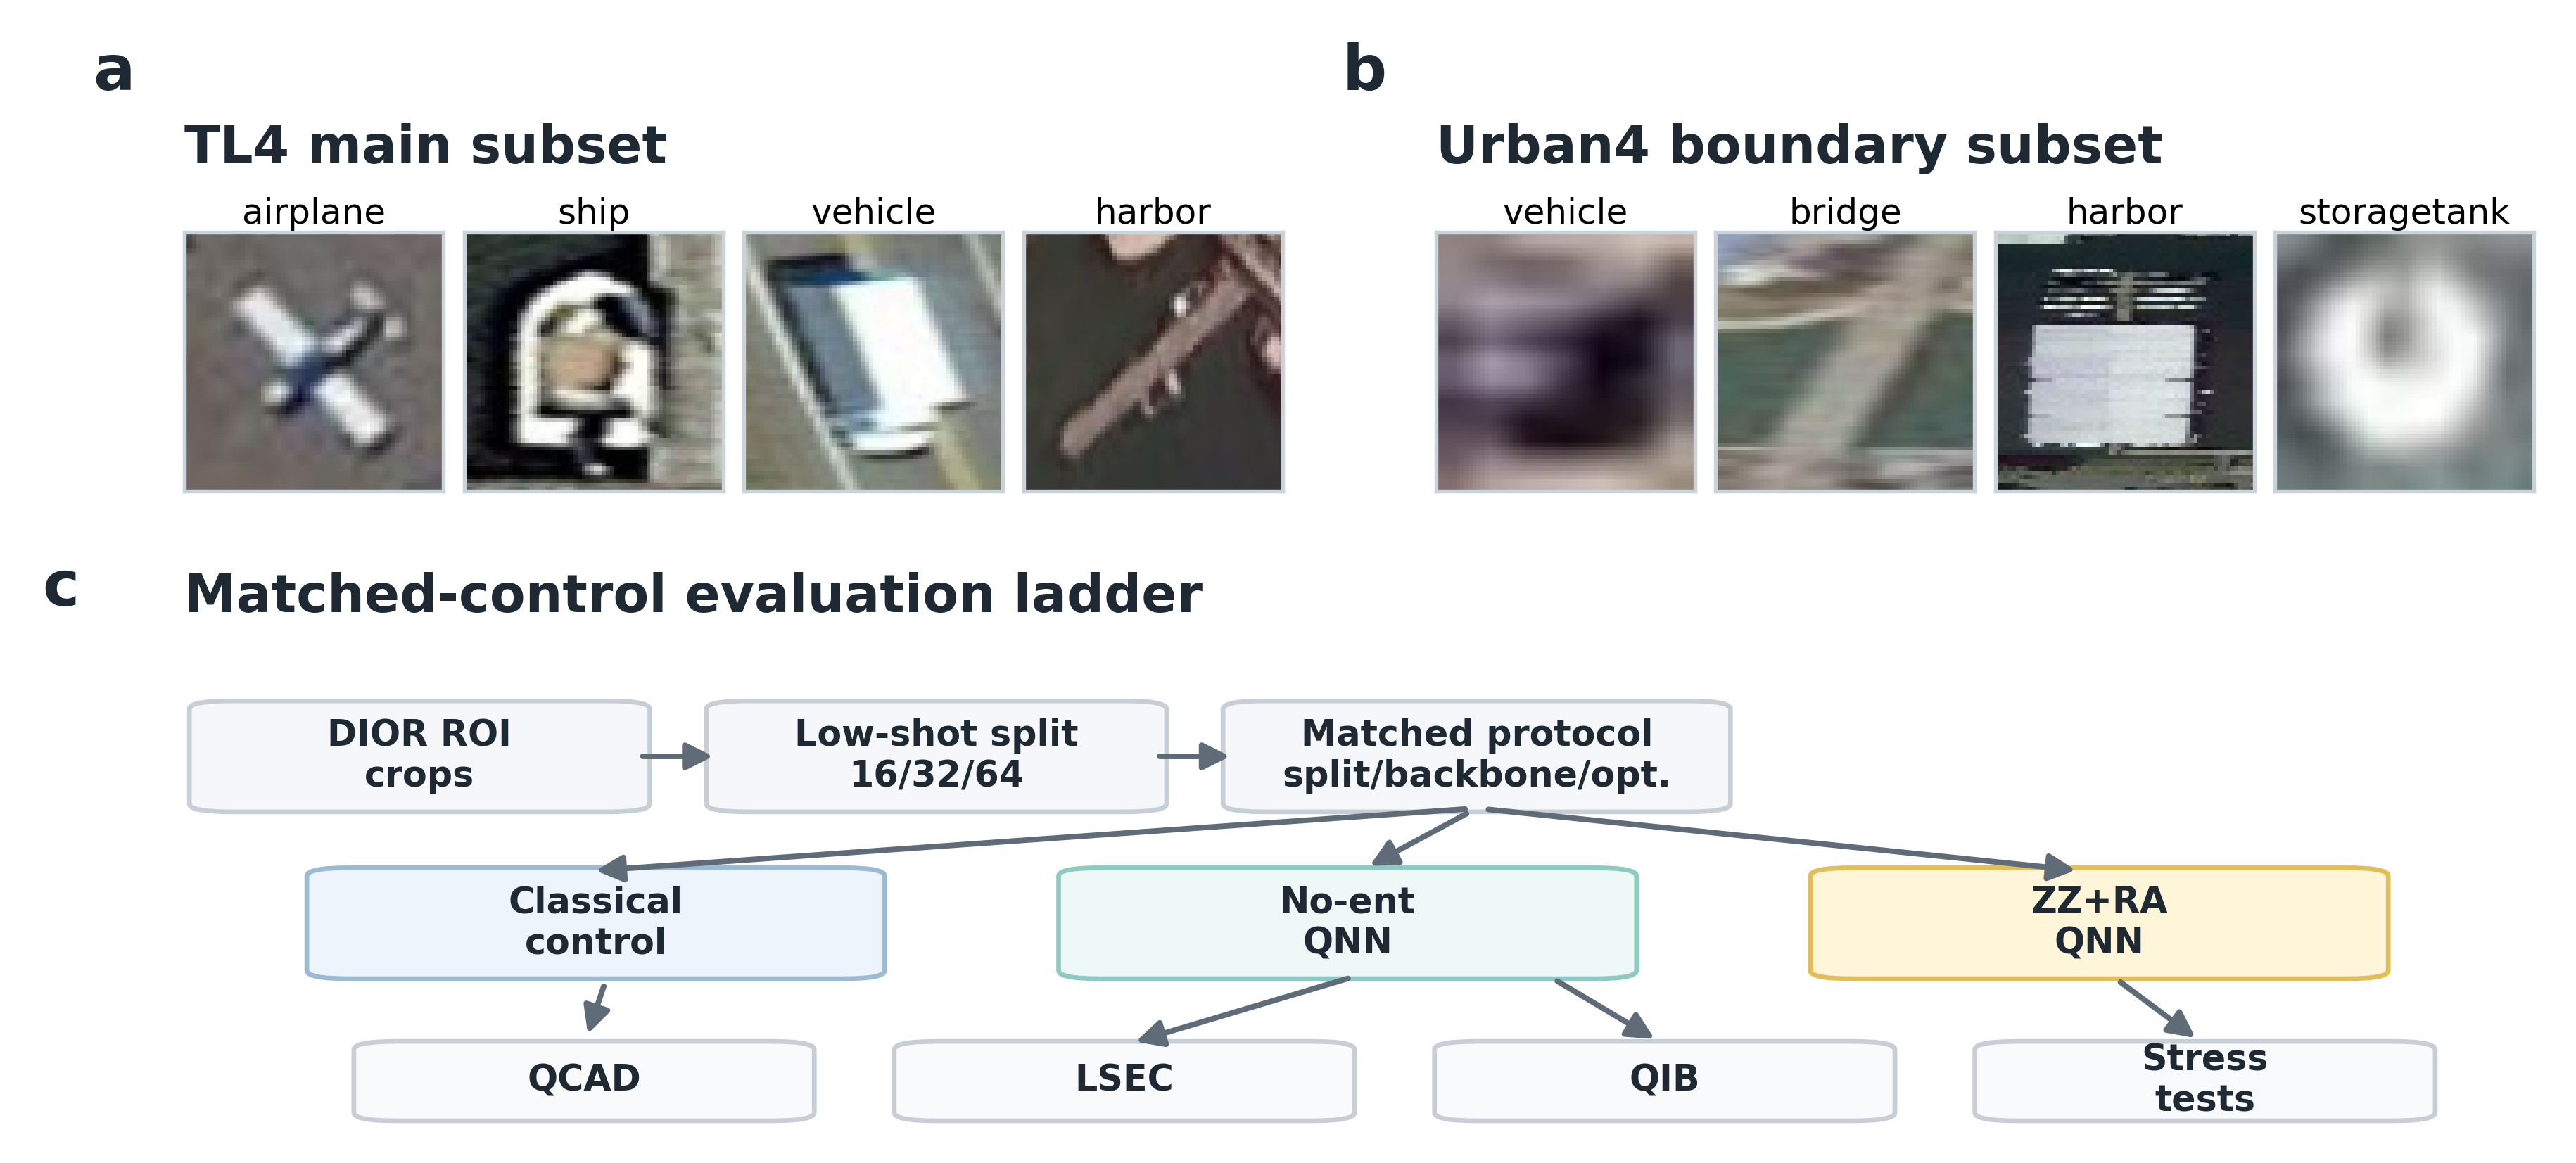
\includegraphics[width=0.96\textwidth]{fig1_study_design_overview}
\caption{Study design. (a) Representative ROI crops from the \TL{} subset used as the main low-shot regime. (b) Representative ROI crops from the \URB{} subset used as the cross-subset boundary check. (c) Matched-control evaluation ladder for comparing the classical branch, no-entanglement QNN, and ZZFeatureMap+RealAmplitudes QNN under a shared protocol.}
\label{fig:study_design}
\end{figure*}

\section{Experimental Protocol}
\subsection{Data and Subsets}
ROI crops are constructed from DIOR object annotations while preserving the original training/validation/test partitions. Per-class train/test counts in the retained full pools range from 3,850/809 to 40,450/11,094 in \TL{} and from 2,293/824 to 27,874/6,255 in \URB{}, whereas the low-shot protocol samples only 16/32/64 training examples per class. The main \TL{} subset contains airplane, ship, vehicle, and harbor. A second subset, \URB{}, contains vehicle, bridge, harbor, and storagetank and is used as a cross-subset boundary test. The \TL{} subset was fixed after exploratory screening and then reevaluated under the seven-seed protocol; the resulting claim is therefore limited to this regime.

\subsection{Models and Training}
Four variants are compared. The lightweight CNN baseline maps a 64-D feature vector to four logits. The matched classical hybrid control shares the same backbone, projection, concatenation, fusion layer, residual logits, and optimizer schedule as the quantum models, but replaces the quantum branch with a classical branch. The no-entanglement QNN uses a four-qubit $R_y$ data-reuploading circuit and outputs four $Z$ expectation values. The ZZ+RealAmplitudes head uses a one-repetition ZZFeatureMap and a one-repetition RealAmplitudes ansatz. Before quantum encoding, both QNNs scale the projected input by $\tanh(x)\pi/2$.

The main protocol uses $64\times64$ images, \texttt{train\_light} augmentation, Adam, a learning rate of $10^{-3}$, weight decay of $10^{-4}$, cosine scheduling with one warmup epoch, gradient clipping at 1.0, and early stopping with patience of 4. The CNN baseline is trained first, and the hybrid models are warm-started from the corresponding baseline checkpoint. The backbone is frozen for the first two epochs and then fine-tuned with a 0.1 backbone learning-rate multiplier. The primary metric is final test macro-F1.

\subsection{Statistical Testing}
All main comparisons are paired by seed. We report means $\pm$ standard deviations, paired mean differences, two-sided paired Wilcoxon signed-rank $p$ values, paired bootstrap 95\% confidence intervals, and sign counts. Because seven seeds make $p$ values coarse, $p$ values are interpreted together with the direction of $\Delta$ and the paired confidence intervals. The 32-shot, 64-shot, ResNet18, and \URB{} experiments are used as boundary diagnostics rather than as evidence for a universal claim.

\section{Results and Boundary Analysis}
\subsection{Main 16-Shot QCAD Result}
Table~\ref{tab:boundary_summary} provides a compact boundary summary of the matched QNN-control comparisons. It reports the main 16-shot \TL{} result together with the shot-count, backbone, and cross-subset boundary checks, while the full per-condition statistics are reported in Supplementary Table~S1.

On \TL{} with 16 labeled samples per class, the matched classical control obtains $0.3055\pm0.1729$ macro-F1. The no-entanglement QNN reaches $0.5031\pm0.1421$, with $\Delta=+0.1976$, six positive differences among seven paired seeds, Wilcoxon $p=0.03125$, and a paired bootstrap 95\% CI of $[+0.0766,+0.3271]$. The ZZ+RealAmplitudes head reaches $0.4545\pm0.1735$, with $\Delta=+0.1491$, seven positive differences, $p=0.01562$, and CI $[+0.0621,+0.2665]$. Thus, for $\delta=0$, the 16-shot \TL{} small-CNN simulation setting lies inside the QCAD of both QNN heads relative to the matched classical control; the mean gains also exceed a practical-gain reference of $\delta=0.10$.

\begin{table*}[!t]
\caption{BOUNDARY SUMMARY OF MATCHED QNN-CONTROL COMPARISONS}
\label{tab:boundary_summary}
\centering
\scriptsize
\setlength{\tabcolsep}{3pt}
\renewcommand{\arraystretch}{1.08}
\begin{tabular}{@{}p{0.18\textwidth}p{0.29\textwidth}p{0.29\textwidth}p{0.12\textwidth}@{}}
\toprule
Regime & No-ent result & ZZ+RA result & Verdict \\
\midrule
TL4, 16-shot, small CNN & $0.5031\pm0.1421$; $\Delta=+0.1976$ & $0.4545\pm0.1735$; $\Delta=+0.1491$ & Inside QCAD \\
TL4, 32/64-shot, small CNN & $\Delta=+0.0094/-0.0021$ & $\Delta=+0.0018/+0.0001$ & Gain contracts \\
TL4, 16-shot, ResNet18 & $\Delta=-0.0011$ & $\Delta=+0.0051$ & Compressed \\
Urban4, 16-shot, small CNN & $\Delta=-0.0062$ & $\Delta=-0.0582$ & No stable transfer \\
\bottomrule
\end{tabular}
\vspace{1pt}
\parbox{0.92\textwidth}{\footnotesize Note: Full macro-F1 means, sign counts, $p$ values, bootstrap intervals, runtime ratios, and per-condition statistics are reported in Supplementary Table~S1.}
\end{table*}

Fig.~\ref{fig:main_evidence} separates the main 16-shot evidence into four diagnostics. Fig.~\ref{fig:main_evidence}(a) reports the seed-level macro-F1 scores, Fig.~\ref{fig:main_evidence}(b) shows paired QNN-control deltas under the same random seeds, Fig.~\ref{fig:main_evidence}(c) converts per-class performance into F1 deltas to diagnose class-structured gain, and Fig.~\ref{fig:main_evidence}(d) directly visualizes the no-entanglement confusion-matrix improvement over the matched control.

\begin{figure*}[!t]
\centering
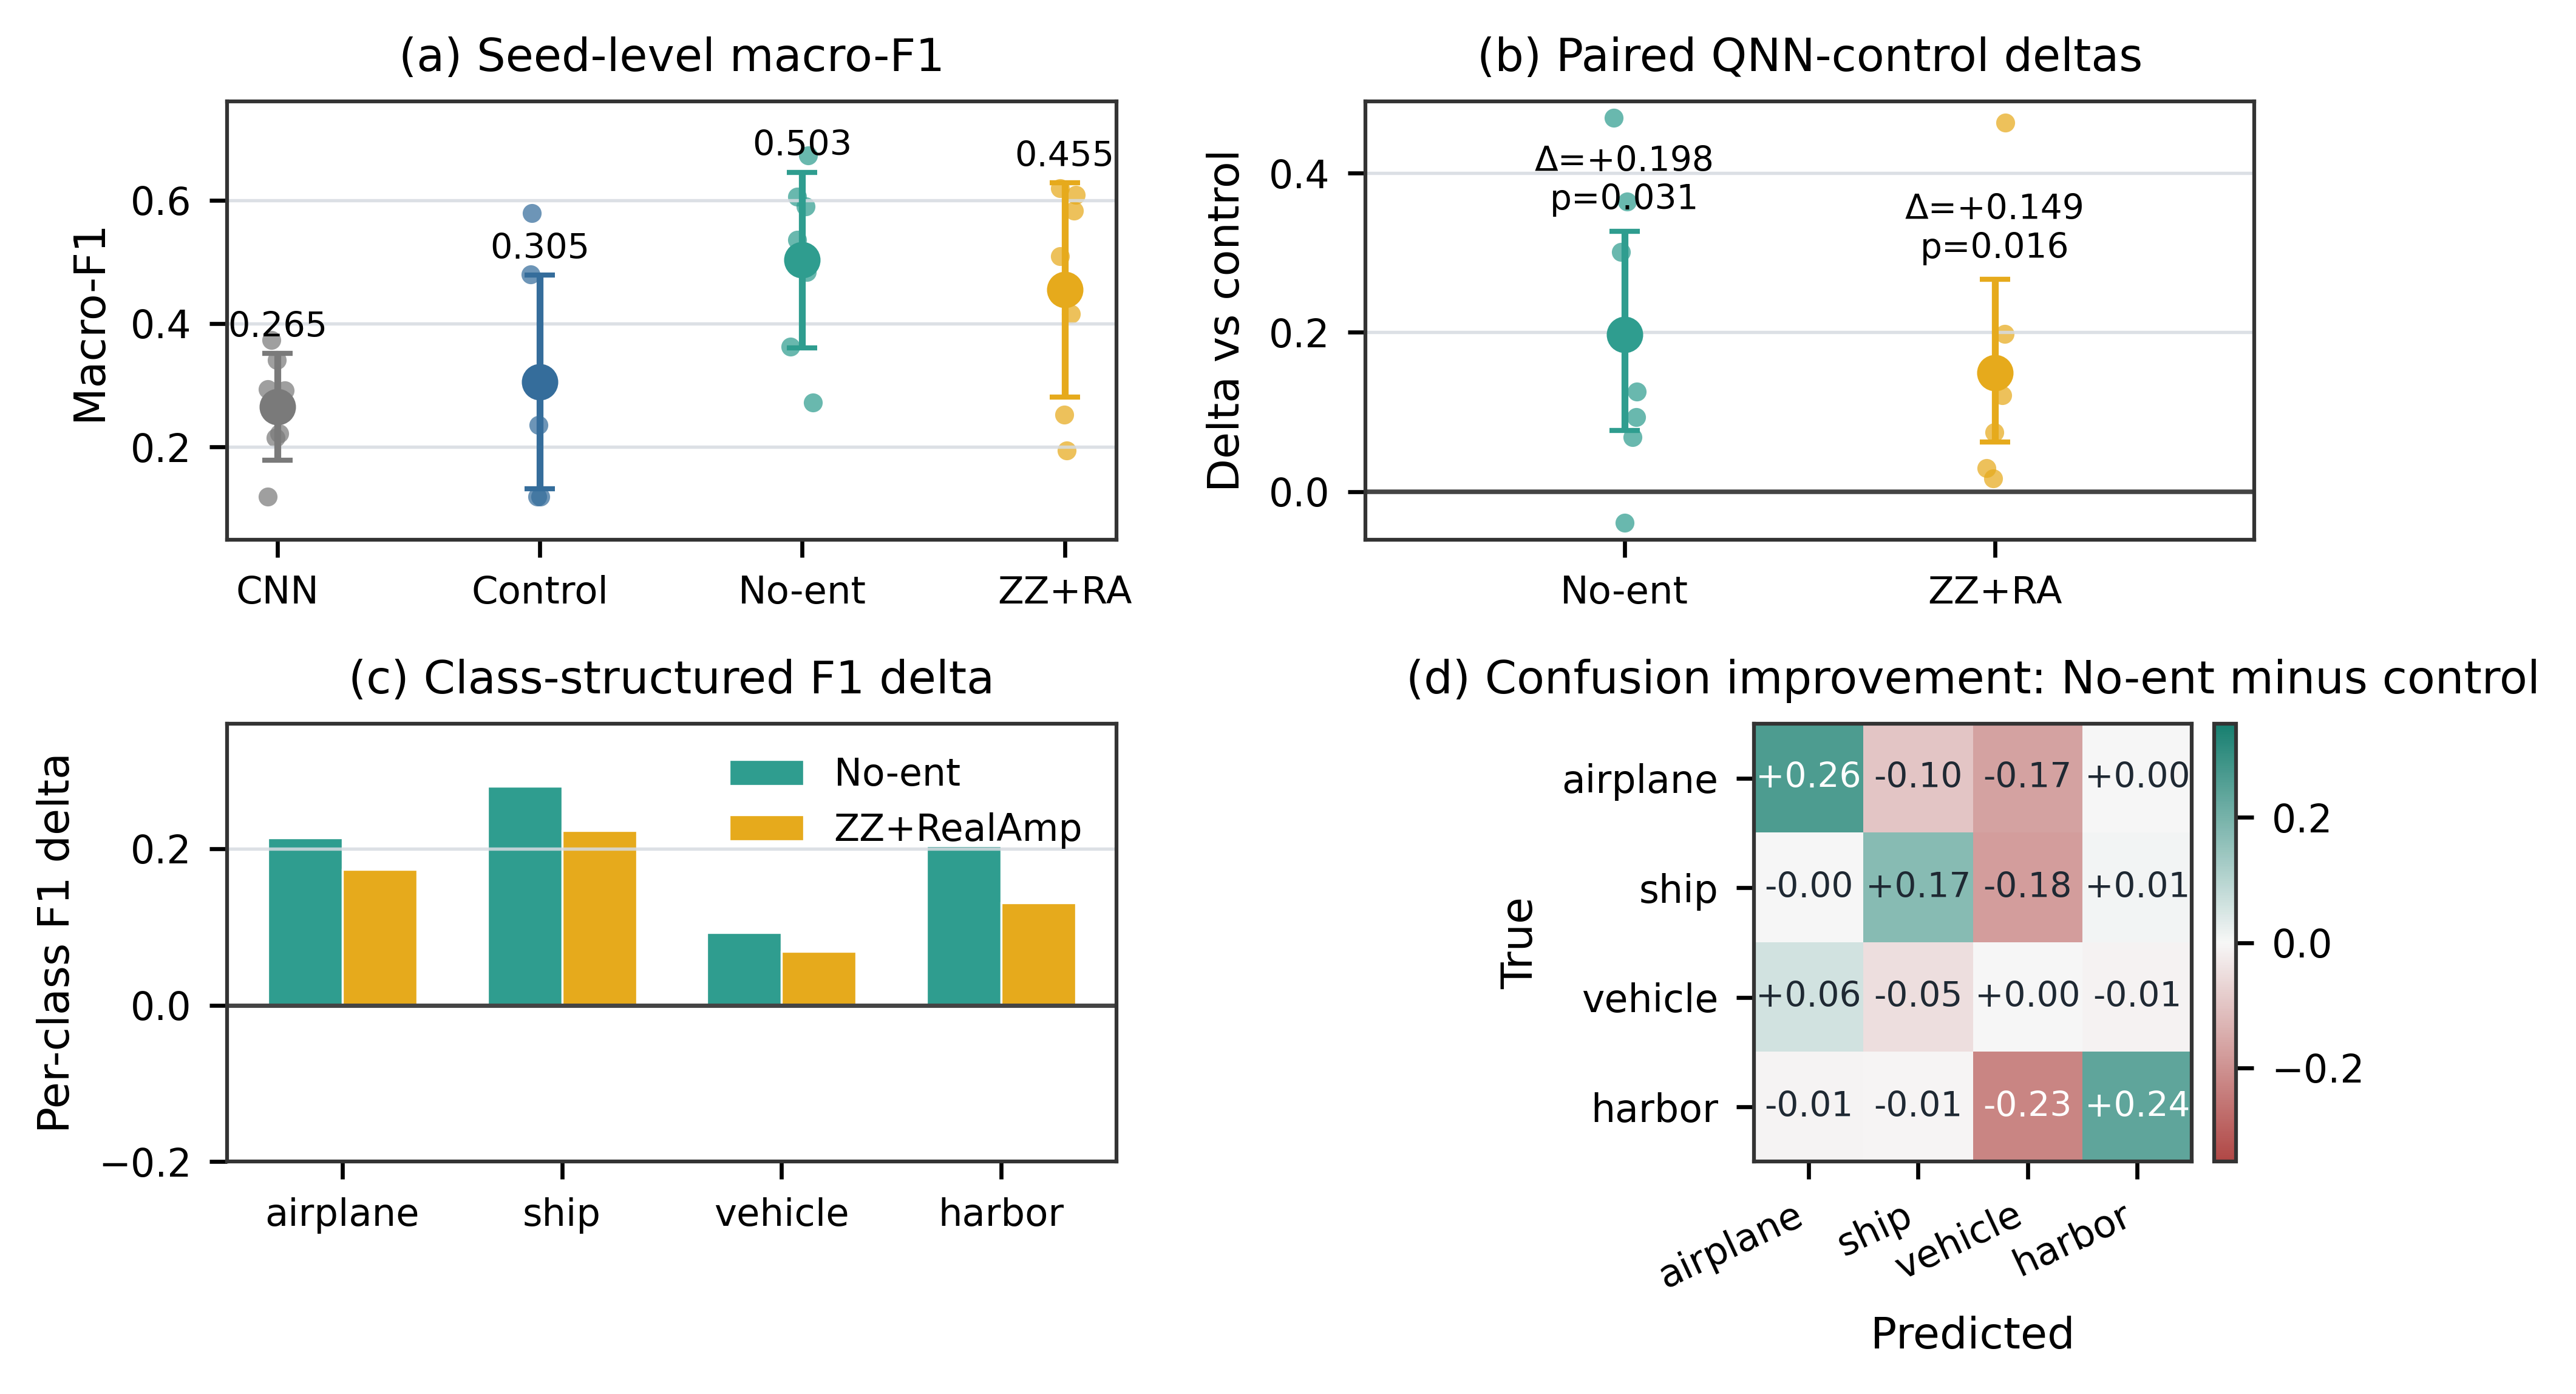
\includegraphics[width=0.96\textwidth]{fig2_main_lowshot_evidence}
\caption{Main 16-shot evidence on \TL{}. (a) Seed-level macro-F1 scores for the CNN baseline, matched control, and two QNN heads. (b) Paired QNN-control deltas. (c) Per-class F1 deltas showing class-structured gain. (d) Confusion-matrix improvement of the no-entanglement QNN over the matched control.}
\label{fig:main_evidence}
\end{figure*}

\subsection{LSEC and Runtime Cost}
The efficiency view changes the circuit ranking. The no-entanglement head has the larger paired mean gain ($+0.1976$) and the lower runtime overhead: 137.20 s versus 59.54 s for the control, corresponding to $\rho=2.30$. The ZZ+RealAmplitudes head remains positive at 16 shots but requires 328.08 s, corresponding to $\rho=5.51$. With $K=4$ and $s=16$, the no-entanglement head therefore has the higher cost-adjusted LSEC. This result does not support a simple ``more entanglement is better'' interpretation; it is more consistent with a compact quantum-head effect.

\subsection{QIB: Class-Structured Rather Than Uniform Gain}
The per-class deltas in Fig.~\ref{fig:main_evidence}(c) and the confusion-improvement pattern in Fig.~\ref{fig:main_evidence}(d) show that the gain is not uniformly distributed across classes. QIB therefore recasts the result as a class-structured inductive bias: the QNN branch helps specific target boundaries more than it improves every class equally.

\subsection{Shot, Backbone, and Subset Boundaries}
Fig.~\ref{fig:boundary_map} summarizes the boundary evidence in two linked views. Fig.~\ref{fig:boundary_map}(a) reports regime-level paired mean macro-F1 gains against the matched classical control, with paired bootstrap 95\% confidence intervals for both QNN heads. Fig.~\ref{fig:boundary_map}(b) isolates the \TL{} small-CNN shot response across 16, 32, and 64 shots/class; the open markers indicate the linear $\Delta=0.10$ crossings used in (3), and the short dotted guide marks their average near 23 shots/class.

Only the \TL{} 16-shot small-CNN condition shows a clearly positive paired gain for both QNN heads, with confidence intervals remaining to the right of zero and mean gains above the $\Delta=0.10$ reference. At 32 and 64 shots the gains collapse toward zero, under ResNet18 they remain near zero, and in \URB{} they do not transfer stably. The observed gain should therefore be read as a simulation-side low-label regime effect rather than a general remote sensing quantum advantage.

\begin{figure*}[!t]
\centering
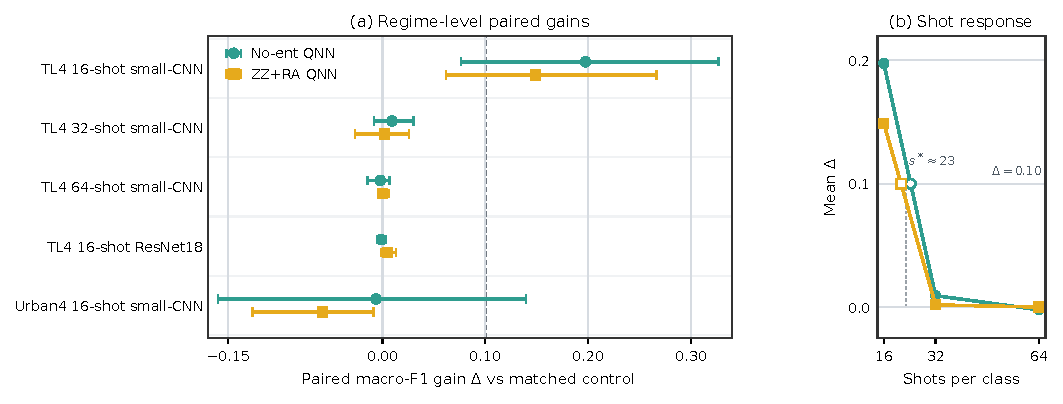
\includegraphics[width=0.96\textwidth]{fig3_journal_boundary_map}
\caption{Boundary evidence across regimes. (a) Paired mean macro-F1 gains of the no-entanglement and ZZ+RealAmplitudes QNN heads relative to the matched classical control; horizontal intervals denote paired bootstrap 95\% confidence intervals. (b) Shot response on the \TL{} small-CNN setting, showing the contraction of the paired gain from 16 to 64 shots/class. Open markers mark the $\Delta=0.10$ crossings, and the short dotted guide marks their average boundary.}
\label{fig:boundary_map}
\end{figure*}

\section{Conclusion}
This letter revises hybrid-QNN evaluation from raw performance comparison to boundary measurement. QCAD identifies paired advantage over a matched classical hybrid control, LSEC links that advantage to labels and runtime, and QIB describes whether the effect is class structured. The metrics do not depend on a specific circuit or task, but their effective boundaries still require validation across datasets, sensors, circuit families, and deployment contexts.

In the 16-shot \TL{} small-CNN simulation setting, both Qiskit quantum heads outperform the matched control across seven paired seeds. The advantage contracts at 32 shots, vanishes at 64 shots, is compressed by ResNet18, and does not transfer stably to \URB{}. The final claim is therefore deliberately bounded: Qiskit hybrid quantum heads can provide measurable help under this matched-control low-shot protocol, but the effect is constrained by label budget, backbone strength, subset composition, circuit design, optimization, and runtime cost. Future work should predefine more subset families, include stronger frozen-feature controls, and test hardware-aware execution.

\section*{Data and Code Availability}
Code, processed metadata, per-seed CSV files, figure scripts, and reproducibility instructions are available at \url{https://github.com/jerry-neal-wang/qiskit_hybrid_qnn_remote_sensing_release}. DIOR images are not redistributed.

\section*{Acknowledgment}
This work was supported by the Science and Technology Development Program of Jilin Province, China (Grant No. 20250205046GH).

\balance
\begin{thebibliography}{99}
\bibitem{li2020dior} K. Li, G. Wan, G. Cheng, L. Meng, and J. Han, ``Object detection in optical remote sensing images: A survey and a new benchmark,'' \emph{ISPRS J. Photogramm. Remote Sens.}, vol. 159, pp. 296--307, 2020.
\bibitem{cheng2017rsi} G. Cheng, J. Han, and X. Lu, ``Remote sensing image scene classification: Benchmark and state of the art,'' \emph{Proc. IEEE}, vol. 105, no. 10, pp. 1865--1883, 2017.
\bibitem{xia2017aid} G.-S. Xia \emph{et al.}, ``AID: A benchmark data set for performance evaluation of aerial scene classification,'' \emph{IEEE Trans. Geosci. Remote Sens.}, vol. 55, no. 7, pp. 3965--3981, 2017.
\bibitem{helber2019eurosat} P. Helber, B. Bischke, A. Dengel, and D. Borth, ``EuroSAT: A novel dataset and deep learning benchmark for land use and land cover classification,'' \emph{IEEE J. Sel. Topics Appl. Earth Observ. Remote Sens.}, vol. 12, no. 7, pp. 2217--2226, 2019.
\bibitem{xia2018dota} G.-S. Xia \emph{et al.}, ``DOTA: A large-scale dataset for object detection in aerial images,'' in \emph{Proc. IEEE/CVF Conf. Comput. Vis. Pattern Recognit.}, 2018, pp. 3974--3983.
\bibitem{zhu2017deep} X. X. Zhu \emph{et al.}, ``Deep learning in remote sensing: A comprehensive review and list of resources,'' \emph{IEEE Geosci. Remote Sens. Mag.}, vol. 5, no. 4, pp. 8--36, 2017.
\bibitem{qiu2024fewshot} C. Qiu \emph{et al.}, ``Few-shot remote sensing image scene classification: Recent advances, new baselines, and future trends,'' \emph{ISPRS J. Photogramm. Remote Sens.}, vol. 209, pp. 368--382, 2024.
\bibitem{zhang2023gfrod} T. Zhang, X. Zhang, P. Zhu, X. Jia, X. Tang, and L. Jiao, ``Generalized few-shot object detection in remote sensing images,'' \emph{ISPRS J. Photogramm. Remote Sens.}, vol. 195, pp. 353--364, 2023.
\bibitem{biamonte2017qml} J. Biamonte \emph{et al.}, ``Quantum machine learning,'' \emph{Nature}, vol. 549, pp. 195--202, 2017.
\bibitem{cerezo2021vqa} M. Cerezo \emph{et al.}, ``Variational quantum algorithms,'' \emph{Nat. Rev. Phys.}, vol. 3, pp. 625--644, 2021.
\bibitem{mcclean2018barren} J. R. McClean, S. Boixo, V. N. Smelyanskiy, R. Babbush, and H. Neven, ``Barren plateaus in quantum neural network training landscapes,'' \emph{Nat. Commun.}, vol. 9, 4812, 2018.
\bibitem{wang2021noise} S. Wang \emph{et al.}, ``Noise-induced barren plateaus in variational quantum algorithms,'' \emph{Nat. Commun.}, vol. 12, 6961, 2021.
\bibitem{havlicek2019supervised} V. Havl\'{i}\v{c}ek \emph{et al.}, ``Supervised learning with quantum-enhanced feature spaces,'' \emph{Nature}, vol. 567, pp. 209--212, 2019.
\bibitem{schuld2019feature} M. Schuld and N. Killoran, ``Quantum machine learning in feature Hilbert spaces,'' \emph{Phys. Rev. Lett.}, vol. 122, 040504, 2019.
\bibitem{sebastianelli2022circuit} A. Sebastianelli, D. A. Zaidenberg, D. Spiller, B. Le Saux, and S. L. Ullo, ``On circuit-based hybrid quantum neural networks for remote sensing imagery classification,'' \emph{IEEE J. Sel. Topics Appl. Earth Observ. Remote Sens.}, vol. 15, pp. 565--580, 2022.
\bibitem{zhang2023hybrid} Z. Zhang \emph{et al.}, ``Remote sensing image scene classification in hybrid classical-quantum transferring CNN with small samples,'' \emph{Sensors}, vol. 23, no. 18, 8010, 2023.
\bibitem{fan2025hybrid} F. Fan, Y. Shi, T. Guggemos, X. X. Zhu, and X. Zhu, ``Hybrid quantum deep learning with superpixel encoding for Earth observation data classification,'' \emph{IEEE Trans. Neural Netw. Learn. Syst.}, vol. 36, no. 6, pp. 11271--11284, 2025.
\bibitem{wilcoxon1945individual} F. Wilcoxon, ``Individual comparisons by ranking methods,'' \emph{Biometrics Bull.}, vol. 1, no. 6, pp. 80--83, 1945.
\bibitem{efron1979bootstrap} B. Efron, ``Bootstrap methods: Another look at the jackknife,'' \emph{Ann. Statist.}, vol. 7, no. 1, pp. 1--26, 1979.
\end{thebibliography}

\end{document}
